\documentclass[12pt]{article}

\usepackage[utf8]{inputenc}
\usepackage{latexsym,amsfonts,amssymb,amsthm,amsmath,mathtools,textcomp,listings,float}
\usepackage[noend]{algorithm2e}
\usepackage[a4paper,bindingoffset=0.2in,%
            left=0.5in,right=0.5in,top=1in,bottom=1in,%
            footskip=.25in]{geometry}

\SetKwProg{Fn}{Function}{}{end}\SetKwFunction{createplan}{createPlan}
\SetKwProg{Fn}{Function}{}{end}\SetKwFunction{construct}{constructFlightAlongTour}
\SetKwProg{Fn}{Function}{}{end}\SetKwFunction{cutcorner}{cutCorner}
\SetKwProg{Fn}{Function}{}{end}\SetKwFunction{pathpoints}{getPathBetweenPoints}
\SetKwProg{Fn}{Function}{}{end}\SetKwFunction{twoopt}{twoOptTSP}
\SetKwProg{Fn}{Function}{}{end}\SetKwFunction{twooptimprove}{twoOptImprove}
\SetKwProg{Fn}{Function}{}{end}\SetKwFunction{waypoints}{nagigateAlongWaypoints}
\SetKwProg{Fn}{Function}{}{end}\SetKwFunction{maxmove}{maxMoveLength}



\begin{document}


\section*{Drone control algorithm}
The 
\subsection*{Algorithms}
\begin{algorithm}[H]
\DontPrintSemicolon
\KwIn{the start coordinate position of the drone $c$, and $G$, a weighted graph of the sensors and their distances to each other, taking into account obstacle evasion.}
\KwOut{a list of moves M that visits all sensors and return to the starting location}
\Fn(){\createplan{c, G}}{
 T $\gets$ \twoopt{G}\;
 T $\gets$ \twooptimprove{tour}\;
 \Return{\construct{T}}
}\;
\KwIn{a list of points $T$ starting and ending with the drone start position with the rest containing a tour of all of the sensors}
\Fn(){\construct{T}}{
 $c \gets T_0$\;
 $M \gets$ [ ]\;
 \For{$i \in [1, size(T)-1]$} {
  $t \gets T_i$\;
  \If{$i < size(T)-1$} {
   $t \gets$ \cutcorner{$c$, $T_i$, $T_{i+1}$}
  }
  $W \gets$ \pathpoints{c, t}\;
  $M$.add(\waypoints{c, W, 1, \maxmove{c, $W_1$}}) \tcp*{start at 1 since the first is the sensor we have already reached}
  c $\gets$ last(M) \tcp*{update current location to the end of the latest move}
 }
 \Return{M}\;
}
\Fn(){\cutcorner
\;
\caption{Creates a flight plan for the drone which visits all sensors and returns to the start. It first uses a two stage 2-opt heuristic on a pre-generated sensor grapht o generate a tour. It then scans through the tour, constructing a flight plan along a list of waypoints which pathfind around any obstacles using the drone movement rules. Before each step of generating the flight plan, it attempts to ``cut the corner'', taking advantage of the fact that sensors have a 0.0002 range to shorten the route. In the implementation there are many bonus features: the algorithm is run a large number of times, in parallel if possible, and the shortest flight plan is chosen. Depending on the options (default is timed), this continues for a fixed number of iterations or a set amount of time (which can be input as an extra command line argument), after which it stops and chooses the best. }
\end{algorithm}
\begin{algorithm}[H]
\DontPrintSemicolon
\KwIn{the current coordinate position $c$, a list of waypoints $W$, the last of which is the target sensor or end position, the current waypoint number $i$, the number of moves remaining until we declare a potential path invalid $t$}
\KwOut{a list of moves which move the drone along the waypoints into range of the targets, in reverse order}
$D \gets ()$ \tcp*{the set of points that have been examined so far}
\Fn(){\waypoints{c, W, i, t}}{
 \If{$t = 0$} {
  \Return null\;
 }
 \ForEach{offset $\in$ $[0, 10, -10, ..., 170, -170]$}{
  $\theta \gets$ offset + direction from $c$ to $W_i$ rounded to the nearest 10°\;
  $d \gets$ position after moving 0.0003 in the direction $\theta$\;
  \If{$d \in D$}{
   \textbf{continue} \tcp*{try the next offset}
  }
  $D.add(d)$\;
  \If{the line $cd$ collides with an obstacle}{
   \textbf{continue} \tcp*{try the next offset}
  }
  \If{$W_i$ is not the last waypoint and $d$ has line of sight to $W_{i+1}$}{
   $M \gets$ \waypoints(d, W, $i+1$, \maxmove($d$, $W_{i+1}$))\;
   \eIf{$M$ is not null} {
     \Return{$M.add($ a move from c to d in direction $\theta)$}
   }{
    \textbf{continue} \tcp*{try the next offset}
   }
  }
  \If{$d$ is within 0.0002 of the target sensor or 0.0003 of the end position} {
   \Return{$[$Move(c, d, $\theta$, sensor if it is not the end)$]$}
  }
  $M \gets$ \waypoints(d, W, $i+1$, $t-1$)\;
  \If{$M$ is not null} {
   \Return{$M.add($ a move from c to d in direction $\theta)$}
  }
 }
 \Return{null}\tcp*{if none of the offsets worked}
}
\Fn(){\maxmove{c, w}\tcp*[f]{auxiliary function}}{
 \Return $2 + \lceil cw \rceil/0.0003$\;
}
\;
\caption{Recursively finds moves which navigate from waypoint to waypoint, until the target location is reached. The main idea of this algorithm is to move in the direction of a waypoint until we reach it, and then move to the next waypoint, until we reach the target sensor or end position. If the target is an intermediate waypoint located on the corner of a no-fly zone, we determine that we have reached it not with but a range but when the next waypoint is in sight, since the waypoints exist to find paths around obstacles. We also keep track of which points we have examined so far to avoid looping, and stop examining a branch if it takes far more moves than expected, because it went the wrong way or got stuck somehow. If the move we tried hits an obstacle or gets stuck further down the recursive call, we try a different offset from the direction until we find one that works. In most cases, which do not need to avoid any obstacles, this algorithm will progress directly towards the target and terminate very quickly. }
\end{algorithm}

\subsection*{Examples}
what, why?
\begin{figure}[H]
	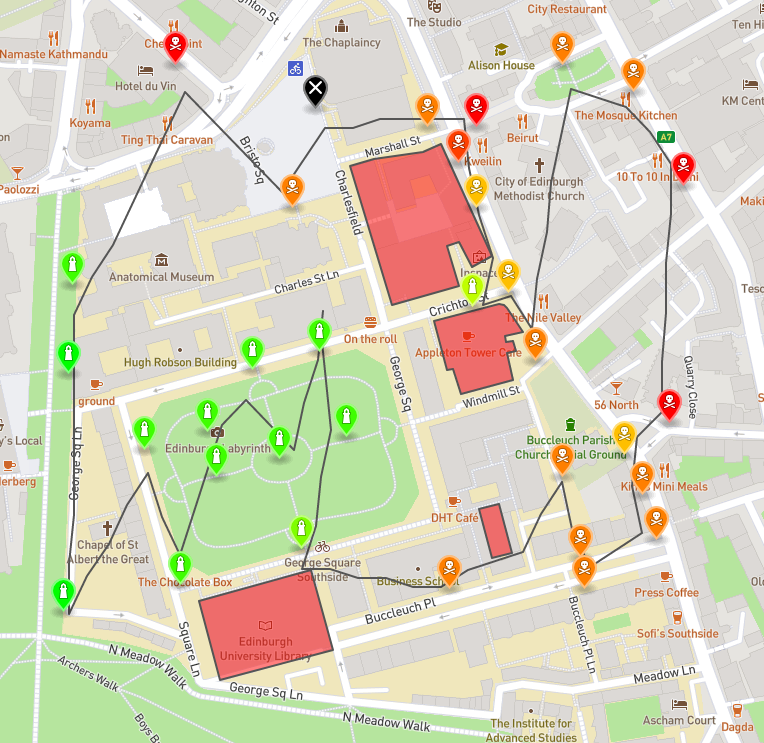
\includegraphics[width=0.5\linewidth]{01-01-2020}
	\caption{01/01/2020}
	\label{fig:1}
\end{figure}


\end{document}